%!TEX root=../seke.tex
% mainfile: ../seke.tex

\begin{table}[t]
  \centering

  {\footnotesize
  \begin{tabular}{r | c c c}
                           Schema & Tables & Columns & Constraints \\ \hline
    BioSQL                        & 28     & 129     & 186 \\
    Cloc                          & 2      & 10      & 0 \\
    iTrust                        & 42     & 309     & 134 \\
    JWhoisServer                  & 6      & 49      & 50 \\
    NistWeather                   & 2      & 9       & 13 \\
    NistXTS748                    & 1      & 3       & 3 \\
    NistXTS749                    & 1      & 3       & 3 \\
    RiskIt                        & 13     & 57      & 36 \\
    UnixUsage                     & 8      & 32      & 24
\end{tabular}}

  \vspace*{-.05in}
  \caption{Database schemas used in the experiments.}~\label{tab:schemas}
  \vspace*{-.25in}

\end{table}

\vspace{-.05in}
\section{Empirical Analysis}
\vspace{-.05in}

\textbf{Experimental Design}. To gain a full picture of the performance trade-offs, we conducted an experiment for every
configuration of the parameter space (i.e., schema, coverage criterion, data generator, and doubling technique).
Table~\ref{tab:schemas} shows that the experiments focused on nine schemas that contain between 1 and 42 distinct
tables, 3 to 309 columns, and up to 183 constraints. Including all of the test adequacy criteria proposed by McMinn et
al.~\cite{mcminn2015}, the experiments study ``weak'' criteria (i.e., APC, NCC, ICC, and UCC), ``moderately strong''
ones (i.e., ANCC, AICC, and AUCC), and ``strong'' criteria (i.e., CondAICC and ClauseAICC). More details about each
criterion, including its formal definition and relationship to the other criteria, are available in~\cite{mcminn2015}. We
used all six test data generators provided by the {\em SchemaAnalyst} tool for automated test data
generation~\cite{kapfhammer2013}, with four techniques employing a variant of random search and two based on Korel's
alternating variable method. After a restart of the search for suitable test data, all of these data generators could
start with either default or random values.

% GMK NOTE: Can we safely cut this sentence? I don't think that it is absolutely needed (I have already revised it)

% In an effort to ensure good picks for parameters, we also conducted preliminary experiments.

In our study, we set $\mathit{tolerance}$ to $0.40$ and $\mathit{lookback}$ to $4$. These values were chosen by
performing doubling experiments on various algorithms, with known worst-case time complexities, and observing that the
ratio converged to the correct value with this configuration.  We set $\mathit{minimum}$ to $20$ after observing that
\textit{SchemaAnalyst} stopped displaying constant behavior after around 5 doubles.  Preliminary studies showed that,
while experiments for fast configurations could be completed in less than an hour, slower configurations required days.
Since there are over four thousand possible configurations, the study needed a substantial amount of computational
resources.  As a solution, we ran the experiments on a high-performance computing (HPC) cluster containing 195 worker
nodes of various hardware configurations, ranging from 12 to 16 CPU cores and 24 to 256 GB of memory, and using the
64-bit Redhat operating system.

% GMK NOTE: It would be better to call this a tree model instead of a regression tree -- the word regression is also
% used in the software testing literature to have a different meanining.

% Regression tree
% Belongs with results_trees, but must be here for page placement within the paper

\begin{figure*}[t!]
\vspace*{-.2in}
\centering
\begin{subfigure}{0.5\textwidth}
  \centering
  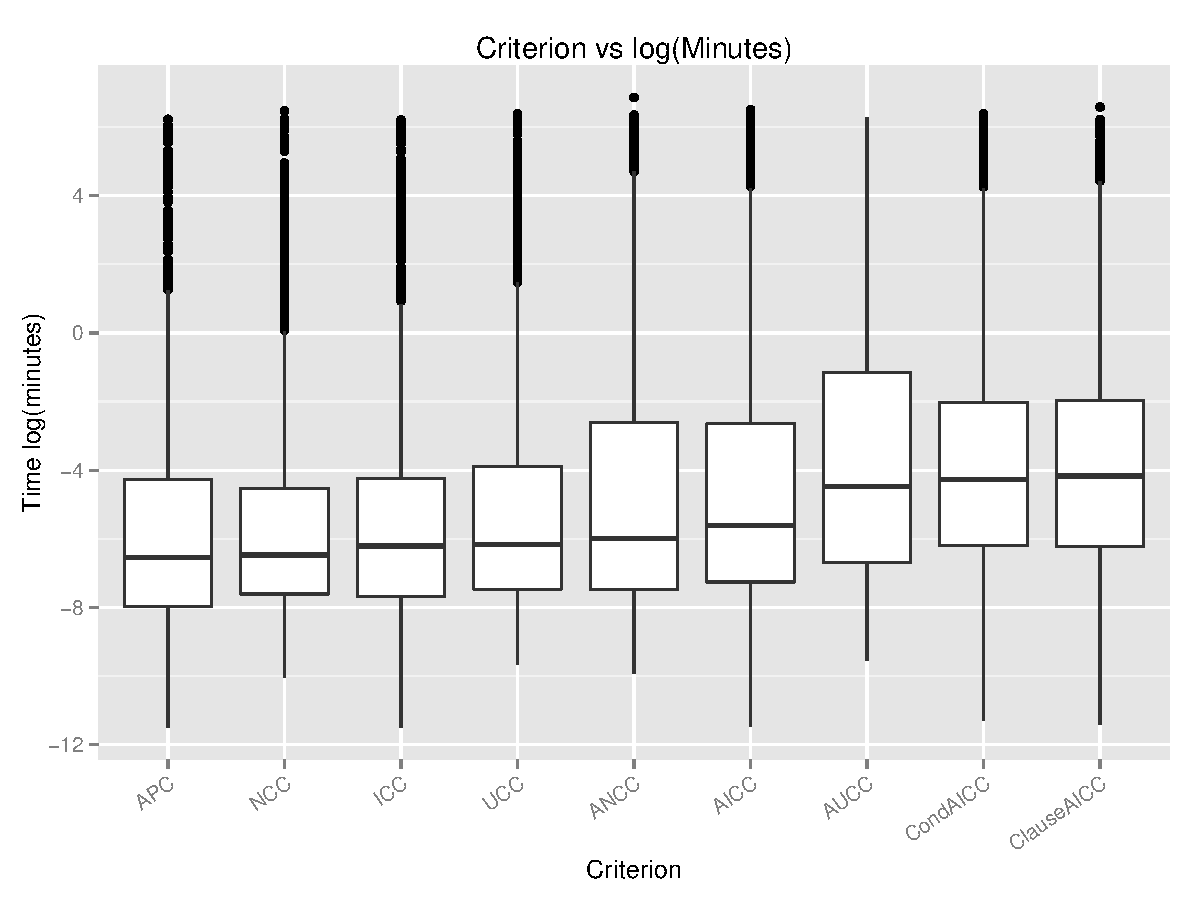
\includegraphics[width=.8\linewidth]{diagrams/CriterionOrder.pdf}
  \caption{Coverage criterion versus runtime in minutes.}
  \label{fig:crites}
\end{subfigure}%
\begin{subfigure}{0.5\textwidth}
  \centering
  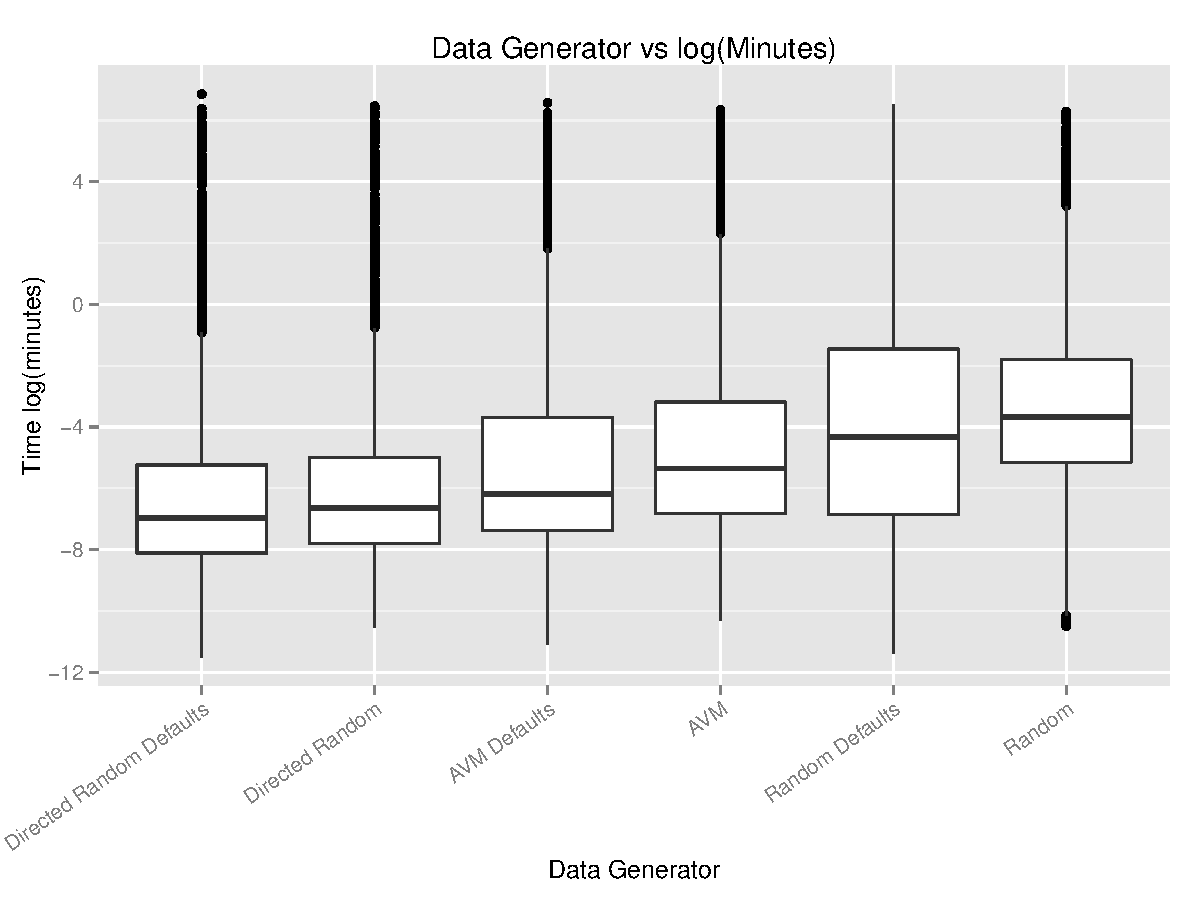
\includegraphics[width=.8\linewidth]{diagrams/DataGeneratorOrder.pdf}
  \caption{Data generator versus runtime in minutes.}
  \label{fig:datas}
\end{subfigure}
\label{fig:bwplots}
\caption{Box and whisker plots for criterion and data
  generator.}
  \vspace*{-.15in}
\end{figure*}

